\section{Introduction}


\begin{figure}[t]
\centering
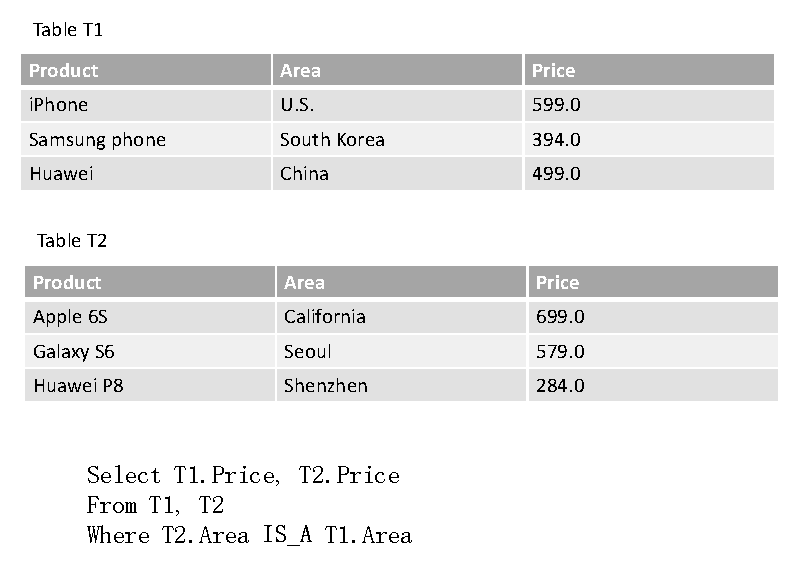
\includegraphics[width=0.45\textwidth]{figures/productexample}
 \caption{Examples to illustrate approximate joins}
\label{fig:autocompletion}
\end{figure}


Strings form a fundamental data type in computer systems and string searching has been extensively studied since the
inception of computer science. String similarity search takes a set of strings and a query string as input, and outputs all
the strings in the set that are similar to the query string. A join extends the notion of similarity search further and require
all similar string pairs between two input string sets to be reported. Both similarity search and similarity join are
central to many applications such as data integration and cleaning.

 Taxonomies are sets of is-a hierarchies, which allow aggregating low level data items into higher level concepts. For instance, they found application in (i) mining recurrent high level associations among data as well as their temporal changes [9], [10], [11] and [12], (ii) discovering flipping correlations, i.e., patterns whose correlation flips positive to negative (or vice versa) when generalizing data items at higher abstraction levels [13], and (iii) performing social data disambiguation and analysis [14], [15], [16] and [17]. However, to the best of our knowledge, the integration of taxonomy information in data used for classifier training has never been investigated so far.




Given two strings, $s_1$ and $s_2$, we return three possible relationships between $s_1$ and $s_2$: hypernym, hyponym, mixed. For example, ``California, U.S.'' is a hyponym of ``U.S.'', ``Egypt'' is the same as ``Egypt, Africa Northern'' and ``Egypt'' is a hypernym of ``Africa''. For more examples: ``Egypt, Algeria'' is a hyponym of ``Africa Northern''.

There are two related problems: string join with taxonomy and string similarity join with taxonomy

The leave behind two intriguing questions:

1. How to efficient process string joins with taxonomy? And for multiple joins.


2. How to process the similarity joins and multiple-way similarity joins?  This question becomes increasingly urgent nowadays with the arrival of big data.

%\begin{problem}(String measure with taxonomy). Given two strings $s_1$ and $s_2$ and a taxonomy $T$, how to measure the similarity between $s_1$ and $s_2$ based on T?
%\end{problem}
%\begin{problem}(String joins with taxonomy). Given a string $p$$\in$
%$\Sigma^*$, an integer k, and a synonym set $\mathbb{R}$,  .
%\end{problem}




\subsection{Novelty and contributions}


\smallskip


Our contributions are as follows.

\noindent \textbf{Introduction of string joins with taxonomy}. We introduce a new problem to utilize the taxonomy for the string joins in databases, which has application in data integration and data cleansing.

\noindent \textbf{Optimal algorithms for string joins} We introduce a holistic algorithm for multiple string joins.

\noindent \textbf{Introduction of approximate string joins with taxonomy}: Provide three relationships Hyper, Hypo and mixed similarity.

\noindent \textbf{Novel algorithms for approximate string joins}


Finally, we perform experiments to evaluate our results and show the benefits of proposal algorithms.


\smallskip

The rest of this paper is organized as follows. Section 2
provides the necessary definitions, formulates . Section
3 includes our algorithm for exact joins with taxonomy. In Section 4, we study
the approximate string join, proposing our solution, analyzing its approximation
ratio, and presenting our similarity join algorithms.
Our experiments are presented in Section 5. Finally,
Section 6 concludes with a discussion about future work.